% This .tex file was created by Ray Goerke and Henry Ngo for the
% UBC Physics Society Latex Tutorial Session 2009.  Feel free to
% use this as a reference or template for your own .tex files.

%---------------------- PREAMBLE ----------------------%

%\documentclass{article}
%\usepackage{amsmath}
\documentclass[twocolumn,10 pt,showpacs,preprintnumbers,amsmath,amssymb]{revtex4-1}%RevTeX4 is the standard APS format
\usepackage{graphicx}%Allows incluing figures in ps (or eps) format
\usepackage{dcolumn}%Align columns on the decimal point
\usepackage{bm}%makes math bold

%---------------- THE ACTUAL DOCUMENT -----------------%

\begin{document}

\title{Latex Session 2010}

\author{Your name here}
\affiliation{Department of Physics and Astronomy, University of British Columbia \\
             6224 Agricultural Road, Vancouver, British Columbia, Canada, V6T 1Z1}

\date{\today}

\begin{abstract}
We demonstrate methods for creating nice-looking PDF's for research
papers including mathematical formulae, figures, tables, and bibliographies 
using \LaTeX !
\end{abstract}

\maketitle

\section{Introduction}

You can use latex to do all of the things word processors can do, like
{\bf bold} and {\it italics}.  We can make fonts that are {\Large bigger} or 
even {\Huge bigger} and also fonts that are really {\tiny small}.

New paragraphs like this on are automatically indented according to the document
class that you declared at the begining of the file.  
      Note that actual indenting in the .tex file is ignored.
  You can start or end a line wherever you want, \LaTeX~ will only start a new 
        paragraph is you leave a blank space.
If you want\\ to end\\ a line early\\ you have to use\\ two backslashes.
        
This document uses the 
revtex4 class, which is the standard for all APS journals. It is also the standard
for PHYS/ASTRO 449, which is why we are using it here. The options in the square
brackets of the \verb_\documentclass_ command define various properties of the
document including number of columns and global text size. If you want to see what
a simpler format looks like, you can comment out the \verb_\documentclass_ 
line in the preamble and uncomment the two lines above it. You will also have to
move the \verb_\maketitle_ command to just before the abstract, and comment out both
lines of the affiliation command, because of the slightly different way the two 
document classes handle titles.

\noindent You can use the \verb_\noindent_ command to force a new paragraph to
not be indented.  Also, notice that above when I wrote \verb_\noindent_, \LaTeX~
did not interpret it as a command, but as text.  To do this I used the 
\verb_\verb_ command.

\section{Equations}

One of the most popular features of \LaTeX~ is the ability to make nice looking
math equations.  Here are some examples: 
\begin{equation}
  \int_\alpha^\beta e^{-\frac{{\Gamma_0}^2\omega b x}{q \sigma \epsilon}}\sin\left(\frac{23}{17}\pi x\right)dx
  \label{random}
\end{equation}
      
Note that if you give your equations labels, then you can reference them in the
text, like this: Eq. \ref{heat} and Eq. \ref{random}.  The advantage of using
these types of references is that they will always refer to the correct equation,
even if you add more in later or rearrange them.

There are no limits to what you can do with \LaTeX equations. You can make matricies
and vectors or whatever you like, just google it.

\subsection{Inline equations}

Sometimes you want to have a short bit of math inside the text, like this:
$h\nu = \hbar\omega$.  To do this you can surround your math with
\$'s.

\subsection{Align}

If you want to have a derivation that take multiple lines and have all the equal
signs line up, we can use the align environment:
\begin{align}
  2x^2 + 3(x-1)(x-2) &= 2x^2 + 3(x^2-3x+2)\\
  &= 2x^2 + 3x^2 - 9x + 6\\
  &= 5x^2 - 9x + 6
\end{align}
Note that with both the \verb_eqaution_ and \verb_align_ environments, if you 
put an asterix after the name in the begin statments 
(e.g. \verb_\begin{align*}_), the equations will not be numbered.  The 
same thing works for sections and subsetions. For example the next section has
no number:

\section*{Floats}

Floats are things that \LaTeX~ will intelligently place within your text.  
The most common types of floats are figures and tables.

\subsection{Figures}

The standard package to use for images is graphicx. We start by creating a
\verb_figure_ environment, then a \verb_center_ environment (note the annoying
use of American spelling...). The figure environment tells \LaTeX~ ``I am a
float, you get to put me somewhere to make efficient use of space!''. The
center environment ensures it's centred in the column. We use the
\verb_\includegraphics_ command to include the actual figure, which should be
in postscript (.ps or .eps) format. Note that options in square brackets allow
you to scale or rotate the image. Lastly we add a caption, and give the figure
a label so we can refer to it in the text (see Figure \ref{exp}).

One problem I noticed while doing this last year was that some Windows latex
compilers as well as the ``direct to pdf'' GNU/linux compiler called \verb_pdflatex_
don't understand postscript, so you have to change some compiler options in
the Windows GUI's or use \verb_latex, dvips, ps2psd_ on GNU/linux.

\subsection{Tables}

Tables in \LaTeX~ can sometimes seem tedious, but they are very flexible.  Note that
to make a table we need two environments: first we need the \verb_table_ environment
to make a float which can contain, among other things, captions, and then we need
the \verb_tablular_ environment to actually define the contents of the table.
Technically you could make a table with just the \verb_tablular_ environment, but
then it would no be placed intelligently like other floats and could not be referenced
like Table \ref{sqr}.
\begin{table}
  \caption{\label{sqr}This is a table}
  \begin{tabular}{|l|r|}
    \hline
    $x$  &  $x^2$\\
    \hline
      1    &  1\\
    \hline
      2    &  4\\
    \hline
      3    &  9\\
    \hline
      4    &  16\\
    \hline
      5    &  25\\
    \hline
  \end{tabular}
\end{table}
\begin{table}
  \caption{\label{trendy}This is a trendy table}
  \begin{tabular}{lr}
    \hline
    \hline
    $x$  &  $x^2$\\
    \hline
      1    &  1\\
    \hline
      2    &  4\\
    \hline
      3    &  9\\
    \hline
      4    &  16\\
    \hline
      5    &  25\\
    \hline
    \hline
  \end{tabular}
\end{table}
Right after the \verb_\begin{tabular}_ command, we define some options about the columns.
I have written \verb_|l|r|_, which means we have two columns, the first is left-aligned,
and the second is right-algined. The vertical lines or `pipes' for us 'Nix nerds mean that
there should be a vertical line on the outsides of the table and separating the columns.
In the content of the table, you should write \verb_\hline_ every time you want to a horizontal
line, and then separate each column with an \&. Also every line that isn't an \verb_\hline_
should be ended by two backslashses.

Table \ref{trendy} shows how you can change some of the above options to make a more 
trendy looking table.

One last comment on floats is that if you don't like where \LaTeX~ puts them and you
really think it should go HERE, then you can force it to by putting \verb_[h]_ right
after the \verb_\begin{table}_ or \verb_\begin{figure}_, like Figure \ref{here}, which
should be right here:
\begin{figure}
  \begin{center}
    \caption{\label{here}This is right here}
    \includegraphics[scale=0.25,angle=-90]{graph.ps}
  \end{center}
\end{figure}

\section{Bibilogarphy}

The best and most flexible way to make a biliography in latex is to use an extention
called Bibtex, but that is somewhat complicated and beyond the scope of this session.
There is a good standard environment which works well as long as you don't want to
get too fancy.  It's called \verb_thebibliography_\cite{author} and you can use it to 
cite things in the text\cite{smith}.  Note that the number will always
be consistent, and will reflect adding or rearranging entries\cite{author}.

\begin{thebibliography}{99}

\bibitem{author} Author, I. N. (Year). Title of the article. Title of the Journal or Periodical, volume number, page numbers.

\bibitem{smith} Smith, L. V. (2000). Referencing articles in APA format. APA Format Weekly, 34, 4-10.

\end{thebibliography}

\end{document}
